\setcounter{page}{24}

\newgeometry{headsep=2mm}
\pagestyle{fancy}
\fancyhead{}
\fancyhead[L]{\textbf{Математический кружок}} 
\fancyfoot{} 
\fancyfoot[L]{\thepage}

\twocolumn
\begin{flushleft}
    
\includegraphics[width=0.1\textwidth]{Screenshot_1123.png}
\end{flushleft}
\vspace{1em}
\begin{flushleft}
\textit{С. Овчинников, И. Шарыгин}
\vspace{1em}

\huge{\textbf{Метод \\бесконечного \\спуска}} 
\end{flushleft}

\vspace{1em}
\noindentКакое иррациональное число самое «старое»? Несомненно, $\sqrt{2}$. Мы не знаeм точно, кто первый доказал иррациональность этого числа, однако мы убеждены, что сделано было это примерно так. 

\vspace{1em}

\noindent\textbf{Доказательство первое}
\vspace{0.3em}

\noindentДопустим, что число $\sqrt{2}$ рационально. Геометрически это означает, что диагональ квадрата длины с соизмерима с его стороной длины $a$, то есть найдутся отрезок длины $d$ и целые числа $m$ и $n$ такие, что $c = dm, a = dn$. Отметим $m-1$ точек на диагонали AC и $n-1$ точек на стороне DC, делящие эти отрезки на кусочки длины $d$. Докажем, что треугольники ACD и КЕС подобны. Отложим на $\abs{AC}$ отрезок $AK$: $\abs{AK} = \abs{AD}$ ; на $\abs{DC}$ - отрезок $DE$: $\abs{DE} = \abs{KC}$. Точки $K$ и $E$ попадут в отмеченные точки (рис 1). Докажем, что треугольники



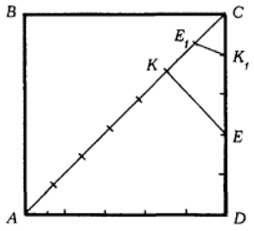
\includegraphics[width=0.3\textwidth]{Screenshot_1124.png}\\
\textbf{Рис. 1.}

\vspace{10em}
\noindent $ACD$ и $KEC$ подобны. Угол $C$ у них общий. Достаточно, значит, проверить равенство $\frac{\abs{KC}}{\abs{EC}}=\frac{\abs{CD}}{\abs{AC}}$.\\
\indent Заметим, что $\abs{KC}= c - a$, $\abs{EC} = 2a - c$. Поэтому $\frac{\abs{KC}^2}{\abs{EC}^2} = \frac{c^2 + a^2 - 2ac}{c^2 + 4a^2 - 4ac}$. Поскольку $c^2 = 2a^2$, $\frac{\abs{KC}^2}{\abs{EC}^2} = \frac{3a^2 - 2ac}{6a^2 - 4ac} = \frac{1}{2} = \frac{\abs{AD}^2}{\abs{AC}^2}$.\\
Таким образом, $\triangle KEC$, подобный $\triangle ACD$, - прямоугольный равнобедренный, и мы можем проделать на его сторонах такое же построение, как на сторонах треугольника $ACD$. Отложим на $\abs{EC}$ Отрезок $EK_1$: $\abs{EK_1} = \abs{KC}$; на \abs{KC} - отрезок $KE_1$: $\abs{KE_1} = \abs{K_1C}$. точки $K_1$ и $E_1$ вновь попадут в точки деления. Треугольник $K_1CE$, снова окажется прямоугольным равнобедренным. Для него мы тем же способом построим треугольник $K_2CE_2$; эту процедуру можно продолжать без конца. При этом треугольники $K_jCE_j$, становятся все мельче, но всякий раз точки $K_j$ и $E_j$, будут попадать в первоначальные точки деления отрезков $AC$ и $CD$. Но ведь этих точек только конечное число! А треугольников $K_jCE_j$ бесконечно много. Это противоречие и доказывает иррациональность $\sqrt{2}$.\\
\indent Прошли века... Появилось алгебраическое доказательство, пожалуй, более простое.

\vspace{1em}

\noindent\textbf{Доказательство второе}
\vspace{0.3em}


\noindent Иррациональность $\sqrt{2}$ означает, что у уравнения $x^2 = 2y^2$ нет решений в натуральных числах $x$, $y$. Допустим, что такие решения есть, и $x = m$, $y = n$ - одно из них.\\
\indent Из уравнения следует, что $m$ - четное число, $m = 2m_1$. Подставляя $m = 2m_1$ в уравнение, получаем $n^2 = 2m^2_1$, то есть $x = n$, $y = m_1$ - тоже решение. Отметим при этом, что $n < m$, $m_1 < n$. Теперь видно, что и $n$ - четное число, $n = 2n_1$, следовательно, $m^2_1 = 2n^2_1$. Таким об-